\documentclass{article}

\usepackage{amsmath,amsfonts,amsthm}
\usepackage{graphicx}
\usepackage{color}
\usepackage{xcolor,pgf,tikz,pgflibraryarrows,pgffor,pgflibrarysnakes}

\usetikzlibrary{fit} % fitting shapes to coordinates
\usetikzlibrary{backgrounds} % drawing the background after the foreground

\tikzstyle{background}=[rectangle,fill=gray!10, inner sep=0.1cm, rounded corners=0mm]
    
\usepgflibrary{shapes}
\usetikzlibrary{snakes,automata}


\usepackage{tikz}
\tikzstyle{nloc}=[draw, text badly centered, rectangle, rounded corners, minimum size=2em,inner sep=0.5em]
\tikzstyle{loc}=[draw,rectangle,minimum size=1.4em,inner sep=0em]
\tikzstyle{trans}=[-latex, rounded corners]
\tikzstyle{trans2}=[-latex, dashed, rounded corners]

\newtheorem{theorem}{Theorem}
\newtheorem{definition}{Definition}
\newtheorem{lemma}{Lemma}
\newtheorem{proposition}{Proposition}
\newtheorem{corollary}{Corollary}
\newtheorem{example}{Example}
\usetikzlibrary{automata,positioning}
\newcommand{\msot}{\textnormal{MSOT}} 
\newcommand{\twst}{\textnormal{2WST}}
\newcommand{\la}{\ensuremath{{\mathrm{la}}}}
\newcommand{\nsst}{\wnsst{}}
\newcommand{\wsst}{\textnormal{SST}} 
\newcommand{\wnsst}{\textnormal{NSST}} 
\usepackage{mathtools}
\usepackage{graphicx}
\usepackage{algorithm}
\usepackage[noend]{algpseudocode}
\usepackage{subcaption}
\makeatletter
\def\BState{\State\hskip-\ALG@thistlm}
\makeatother
\usetikzlibrary{shapes.geometric}
\usetikzlibrary{shapes.arrows}
\usepackage{array}
\usepackage{stmaryrd}
\DeclareCaptionFormat{myformat}{#3}
\captionsetup[algorithm]{format=myformat}

\begin{document}
\title{Discriminating Program Traces using Time}
\author{Saeid Tizpaz Niari, Shyam Sundar Ramamoorthy, Yue Zhang \\ Final Report of Machine Learning (CSCI 5622)  \\ Fall 2016}
\date{}
\maketitle

\section{Introduction}
Different control-flow paths in a program can have varying execution times.
Such observable differences in execution times may be explainable by
information about the program internals, such as whether or not a given function or
functions were called. 
How can a software developer (or security analyst)
determine what internals may or may not explain the varying
execution times of the program? In this project, we consider the problem
of helping such a developer 
or analyst to identify such explanations. 

Given a set of execution traces with observable execution times grouped
into a finite set of labels, a \emph{discriminant} (or a classifier model) is
a map relating each label to a set of features. Such a discriminant model can then be used,
for example, to explain timing differences among program traces based on
its internal features like method calls.  In other words, this problem looks for
distinguishing features among traces that result in
varying execution times.

Crucially, once we can explain the timing
differences in terms of properties of traces (i.e., control-flow paths through
the program), the analyst can use the explanation to diagnose the possible
timing side-channel and potentially find a fix for the vulnerability. 

Our overall approach is to first obtain a set of execution traces
with information recorded about internal features of the input program
along with corresponding execution times. We consider two main
approaches to explain time differences based on the internal features: \\
1- We cluster these training traces based on their overall execution times
to bin them into timing labels. Then, we learn a decision tree discriminant
model from these traces to capture what is common amongst the traces with the
same timing labels and what is different between traces with different labels. \\
2- As the time of execution is a continuous domain (time $\in$ $R$), we can
naturally use regression trees to find discriminant features of the input
program and explain the timing differences. \\
As knowing cluster numbers are important part of our analysis, we apply DBSCAN algorithm
to estimate cluster number. Moreover, we apply other classifier models and measure their
performance.

We present two case studies in identifying and debugging timing
side-channel shown our tools to
perform label clustering and decision tree-discriminant learning. We show that
the decision trees are useful for explaining the timing
differences amongst trace sets and performing this debugging task.

Some technicalities of our approach include that we need to execute both an
instrumented and uninstrumented version of the program of interest: a trace of
the instrumented program is needed to determine which functions are called during
the trace execution, while the execution time of interest is for an uninstrumented
program. Since timing observations are noisy due to many sources of
non-determinism, we also provide this option that each trace is associated with a
\emph{distribution} over the labels.
For instance, a trace may have a label $\ell_1$ with probability $0.9$
and label $\ell_2$ with probability $0.1$.

\section{Motivation Example - existing user enumeration}
In this section, timing side-channel vulnerabilities of a web application is discussed. 
Exploit was found in this application during credentials validation where there is a significant time difference among different scenarios. Figure \ref{user_enumeration-1} shows a sample
authentication scenario where the authentication server checks whether the username
is valid and password is correct. The code snippet shows a sample authentication program.
Based on code, if the user exists in the system, it will check given password. Otherwise, it
will be failed.  

\begin{figure}[t]
    \centering
    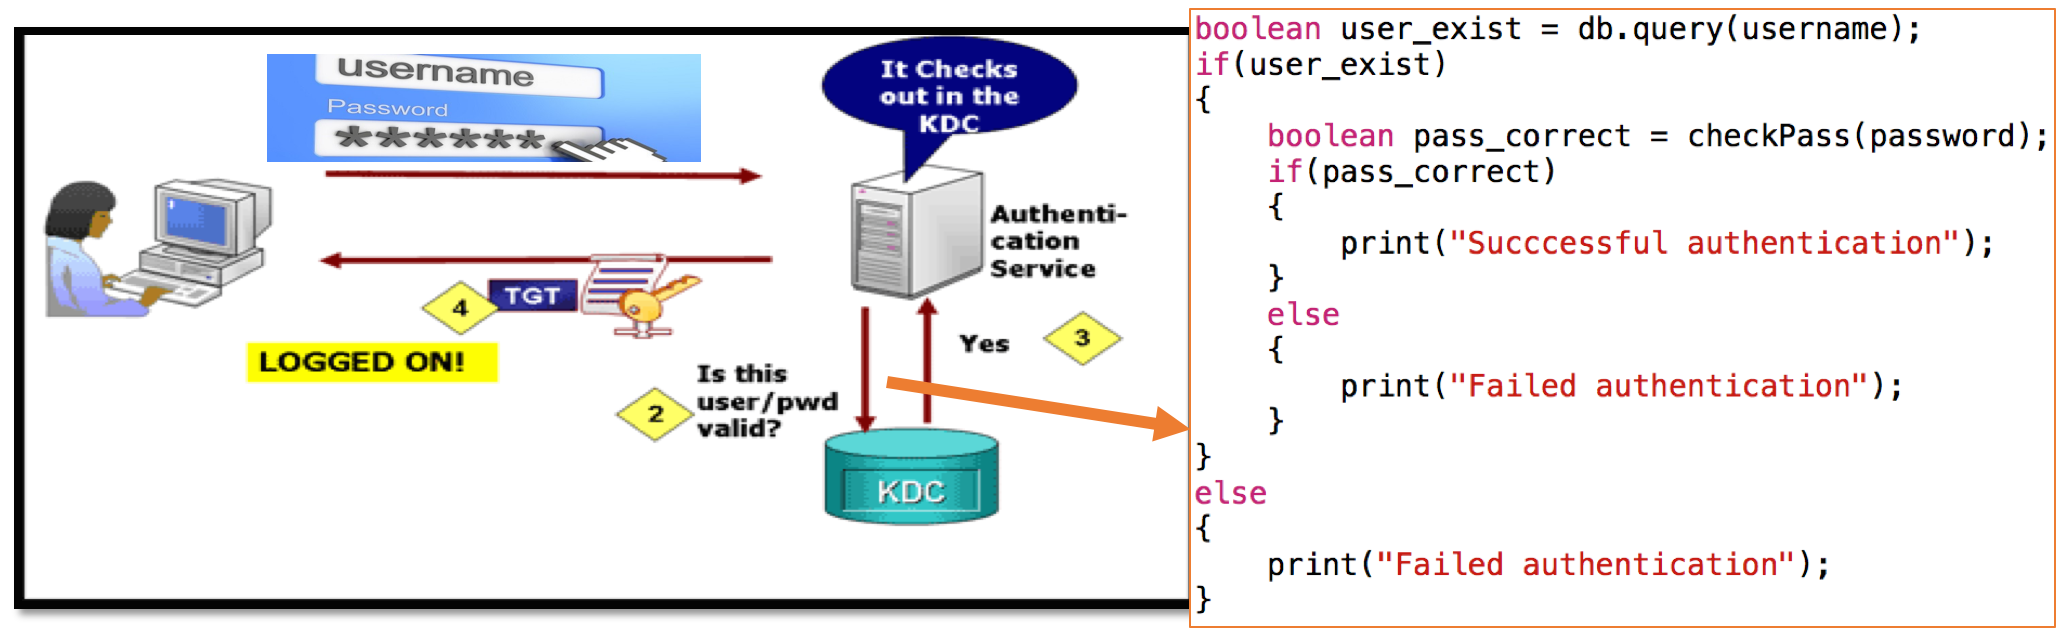
\includegraphics[width=1\textwidth]{User_Enumeration_1}
    \caption{Authentication Scenario for a vulnerable web server}
    \label{user_enumeration-1}
\end{figure}

\subsubsection*{Identifying a Timing Side-Channel with Clustering.}
As an analyst, we issue the server with different username/password combinations. In an
un-instrument version of the authentication server, we generate different valid and invalid
username/password combinations and record execution time for each combination.
Figure \ref{fig:astime} shows scatter plot of the server execution with different username/password 
(each data point corresponds to a unique username/password). The running time is
clustered into $2$ different groups using a standard $k$-means clustering algorithm (k=2). 
This timing difference can indicate a possible side-channel. The scatter shows that for some 
username/password, the download times were roughly $1$ seconds (Cluster\_0), whereas for
some others they were roughly $5$ seconds (Cluster\_1).

\begin{figure}[t]
\centering
\begin{minipage}[b]{0.5\textwidth}
  \centering
  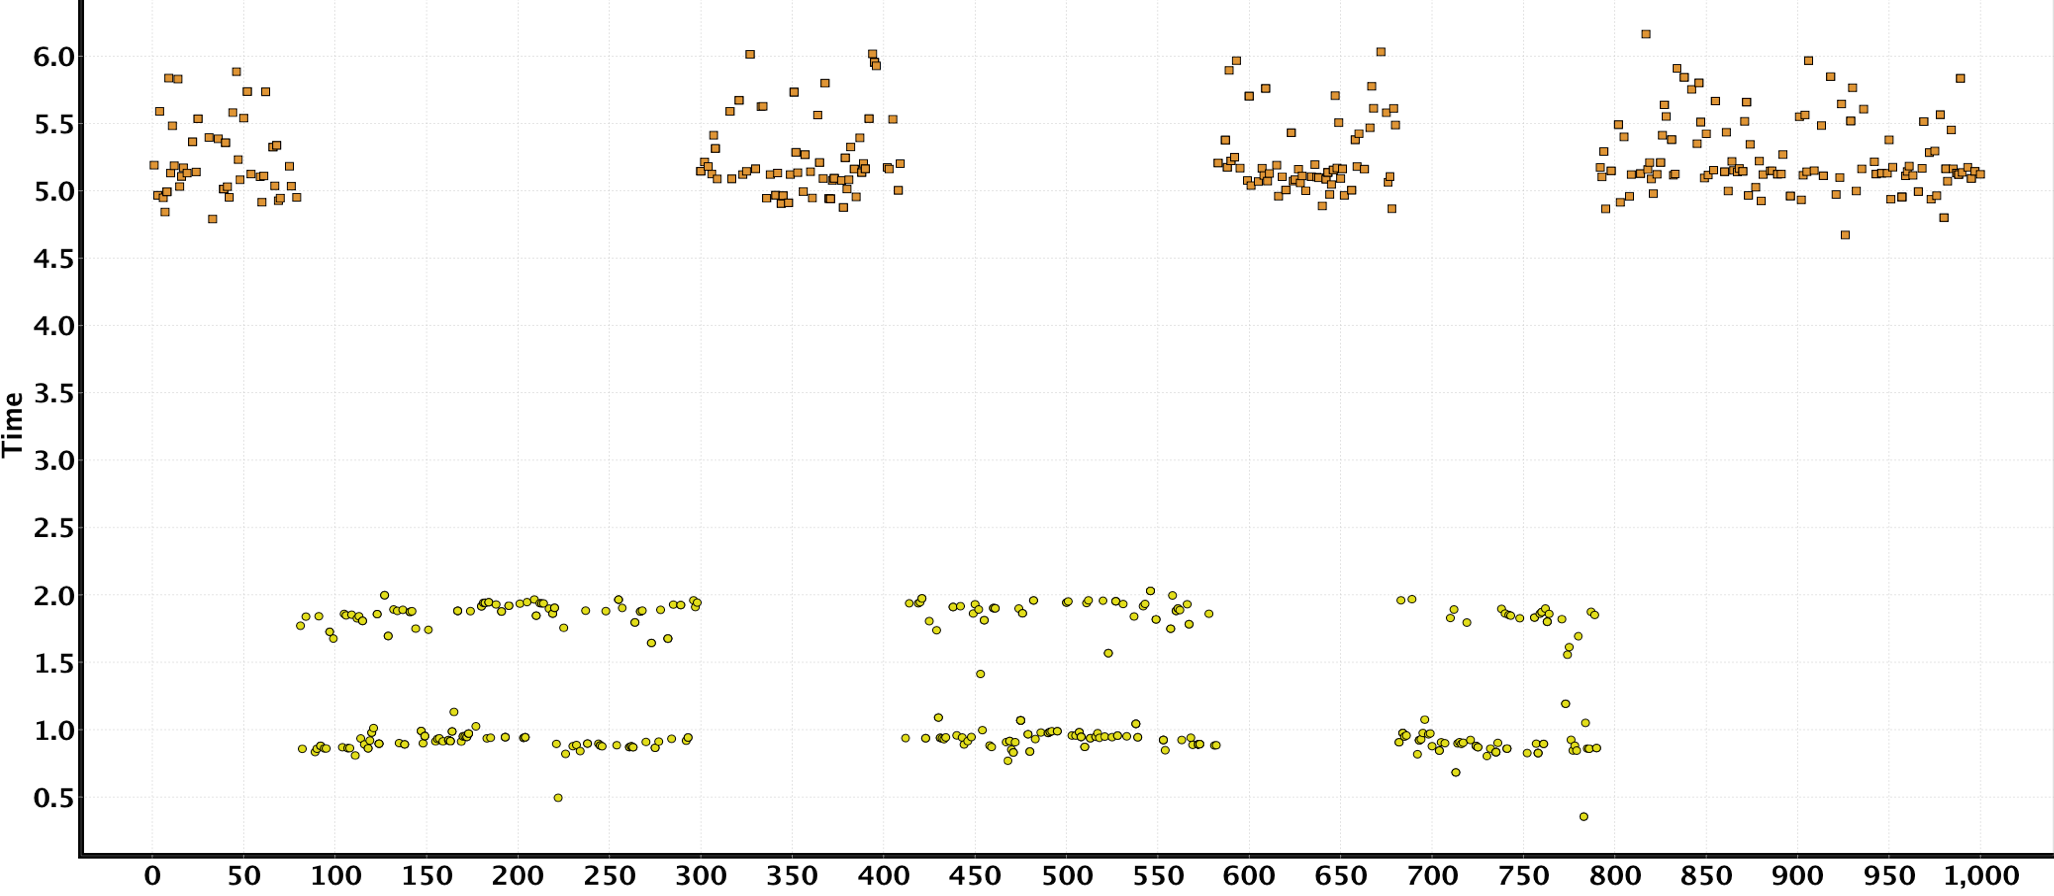
\includegraphics[width=\textwidth]{User_Enumeration_2}
  \caption{Cluster running times from the authentication server to produce labels. The scatter plot shows a differential corresponding to a possible timing side-channel.}
  \label{fig:astime}
\end{minipage}\hfill
\begin{minipage}[b]{0.45\textwidth}
  \centering
  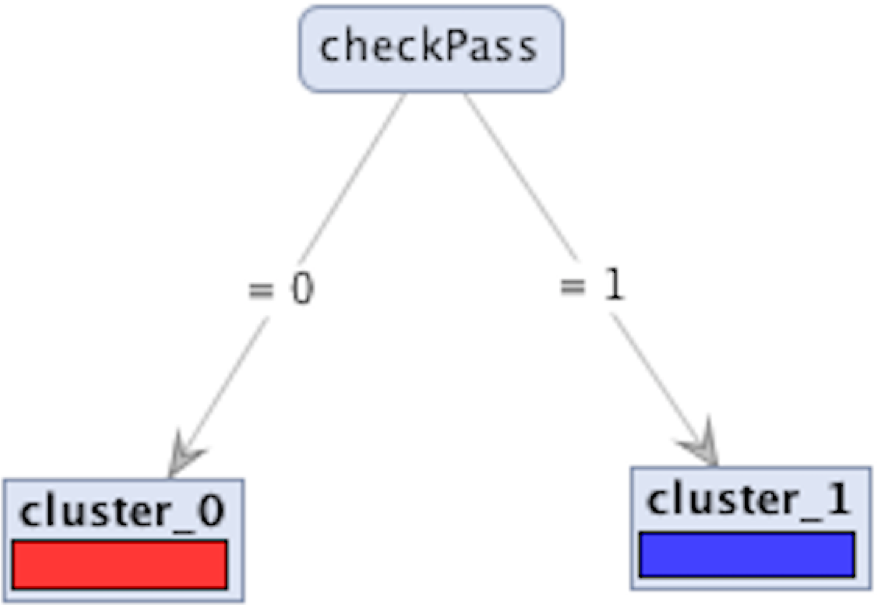
\includegraphics[width=0.6 \textwidth]{User_Enumeration_3}
  \caption{Snippet of a decision-tree discriminant learned from different username/password checking traces using the timing labels from Figure~\ref{fig:astime}.}
  \label{fig:asdectree}
\end{minipage}
\vspace{-1em}
\end{figure}

\subsubsection*{Explaining Timing Side-Channels with Decision Tree Learning.}
Now, we want to explain the time differences based on functions inside the web server.
For this explanation, we run instrumented version of the application with the same input
as the un-instrumented one. The instrumented version will record function calls during the
execution. We assign a label to all traces (each trace is a unique combination of username/password) from the clustering results of previous step. As a result, we generate new data set which includes function calls and labels. Note that each label (Cluster) is corresponding to a
timing range. We use standard \emph{CART} decision tree learning
algorithm to infer a decision tree that
succinctly represents a discriminant
using atomic predicates that characterize
whether or not the trace invoked a particular method (shown in Figure~\ref{fig:asdectree}).
This discriminant model explains that calling checkPass() method is the main reason for
the timing differences. Using this explanation, we can see that the application calls checkPass
for some username/password which take more time than for others. It means that for valid
username it will call checkPass which takes time while for invalid username it will not call this
function. So, the attackers can distinguish valid and invalid username by recording the time of execution.
The possible fix is to call checkPass in the case the username does not exist. 

\section{Motivation Example - SnapBuddy}
In this section, we demonstrate another example to show that the tool can be useful in
identifying timing side-channel vulnerabilities
and suggesting ways to fix them.
We use an application called
SnapBuddy as an example. SnapBuddy is a Java application with 3,071 methods,
implementing a mock social network in which
each user has their own page with a photograph. Figure \ref{snapbuddy-1} shows
a screenshot of SnapBuddy application. Each user logs into system observes the
list of his/her friends, can add new friends, and overview public profile pages of
other users. 

\begin{figure}[t]
    \centering
    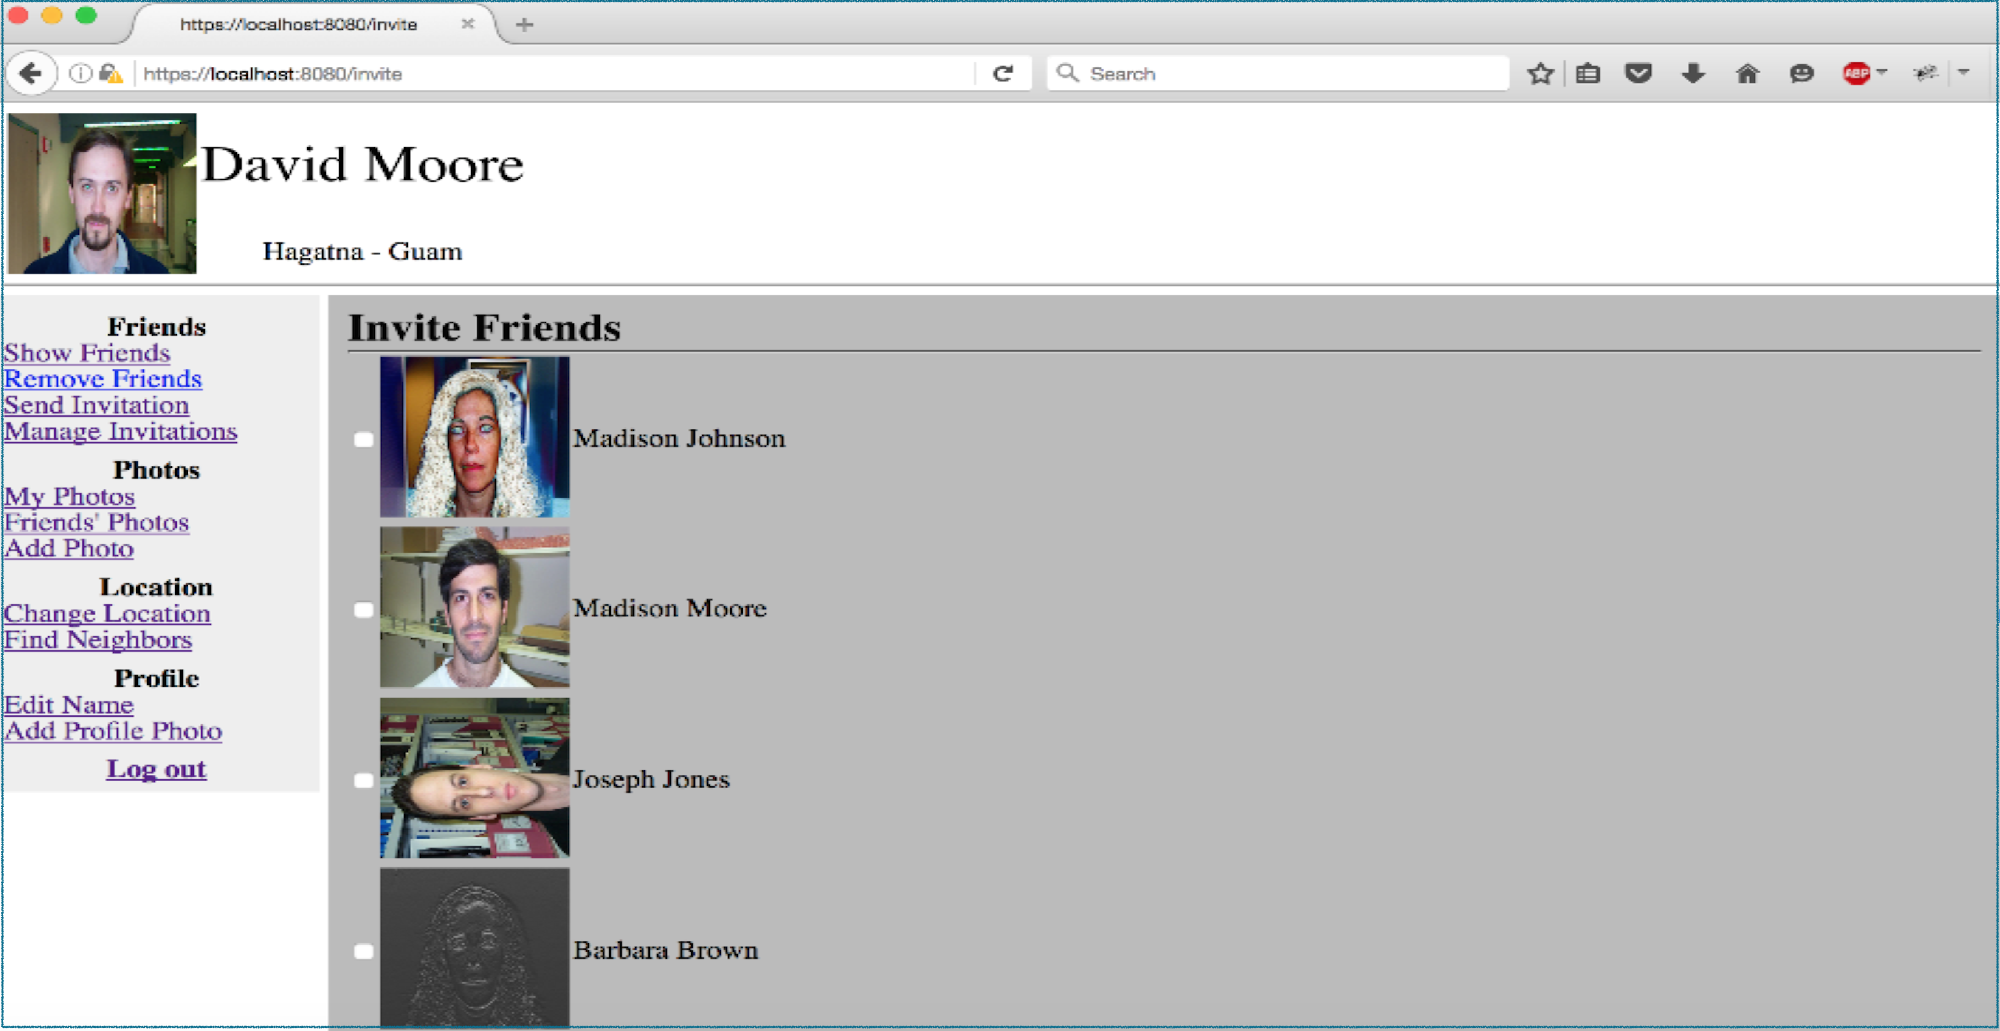
\includegraphics[width=1\textwidth]{snapbuddy-1}
    \caption{A screenshot of SnapBuddy web application}
    \label{snapbuddy-1}
\end{figure}

\subsubsection*{Identifying a Timing Side-Channel with Clustering.}
As we mention, every user can issue download requests to the
public profile page of other users in the system. The public profile
includes the users' public information and their public profile page. 
As an analyst, we record the time to download public pages of all users
in the system. Figure~\ref{fig:sbtime} shows a scatter plot of the running times of
various traces with each trace represented by a point in the figure. The
running times are clustered into $6$ different groups using a
standard $k$-means clustering algorithm and shown using different
colors. We see that for some users, the download times were roughly $15$ seconds, whereas for
some others they were roughly $7.5$ seconds. This significant time differential suggests a
potential timing side-channel if the difference can be correlated with sensitive
program state and thus this differential should be investigated further with the tool.

To see how such a time differential could be a timing side-channel,
let us consider an attacker that
(a) downloads the public profile pages of all users and learns each download time,
and (b) can observe timing between packets by sniffing the
network traffic between legitimate users.
If the attacker observes user Alice downloading the page of another user whose identity
is supposed to be a secret
and sees that the download took approximately $7.5$ seconds, the attacker can infer
that Alice downloaded the page of one of the six users corresponding
to the six red squares in Figure~\ref{fig:sbtime}. The timing
information leak thus helped the attacker narrow down the
possibilities from hundreds of users to six.

\subsubsection*{Explaining Timing Side-Channels with Decision Tree Learning.}
Recall that the analyst downloaded pages
of all the users. Now the same download queries are executed over an
instrumented version of the SnapBuddy server to record the number of
times each method in the application is called by the trace. As a
result, we obtain a
set of traces with their (uninstrumented) overall running times and their
sequence of method calls.

\begin{figure}[t]
\centering
\begin{minipage}[b]{0.47\textwidth}
  \centering
  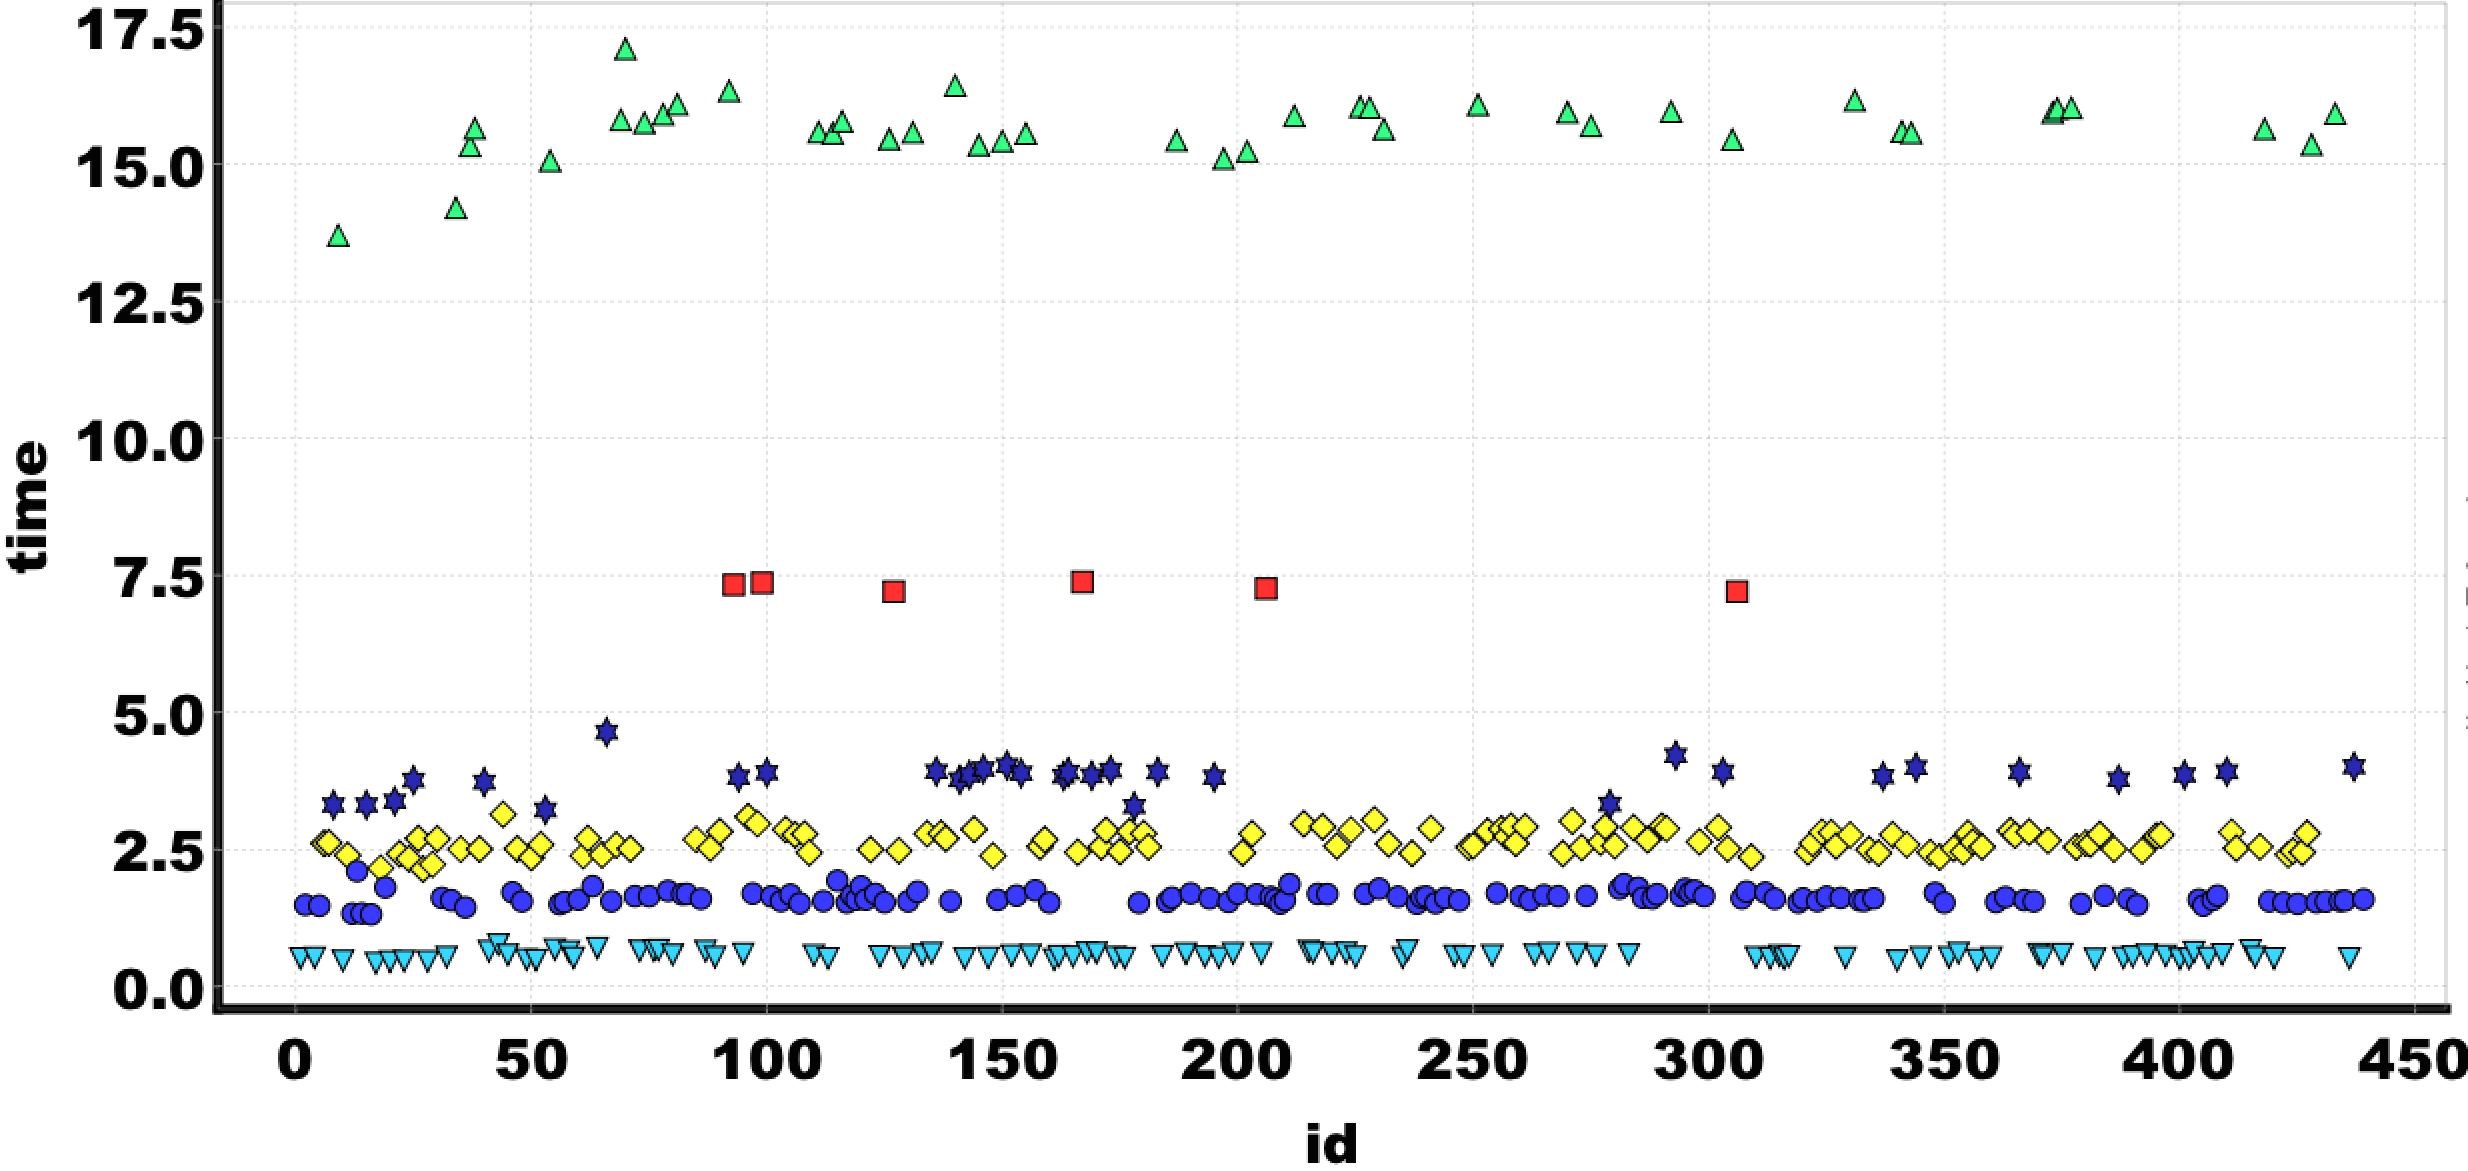
\includegraphics[width=\textwidth]{SnapBuddy_scatter_2}
  \caption{Cluster running times from the SnapBuddy to produce labels. The scatter plot shows a differential corresponding to a possible timing side-channel.}
  \label{fig:sbtime}
\end{minipage}\hfill
\begin{minipage}[b]{0.50\textwidth}
  \centering
  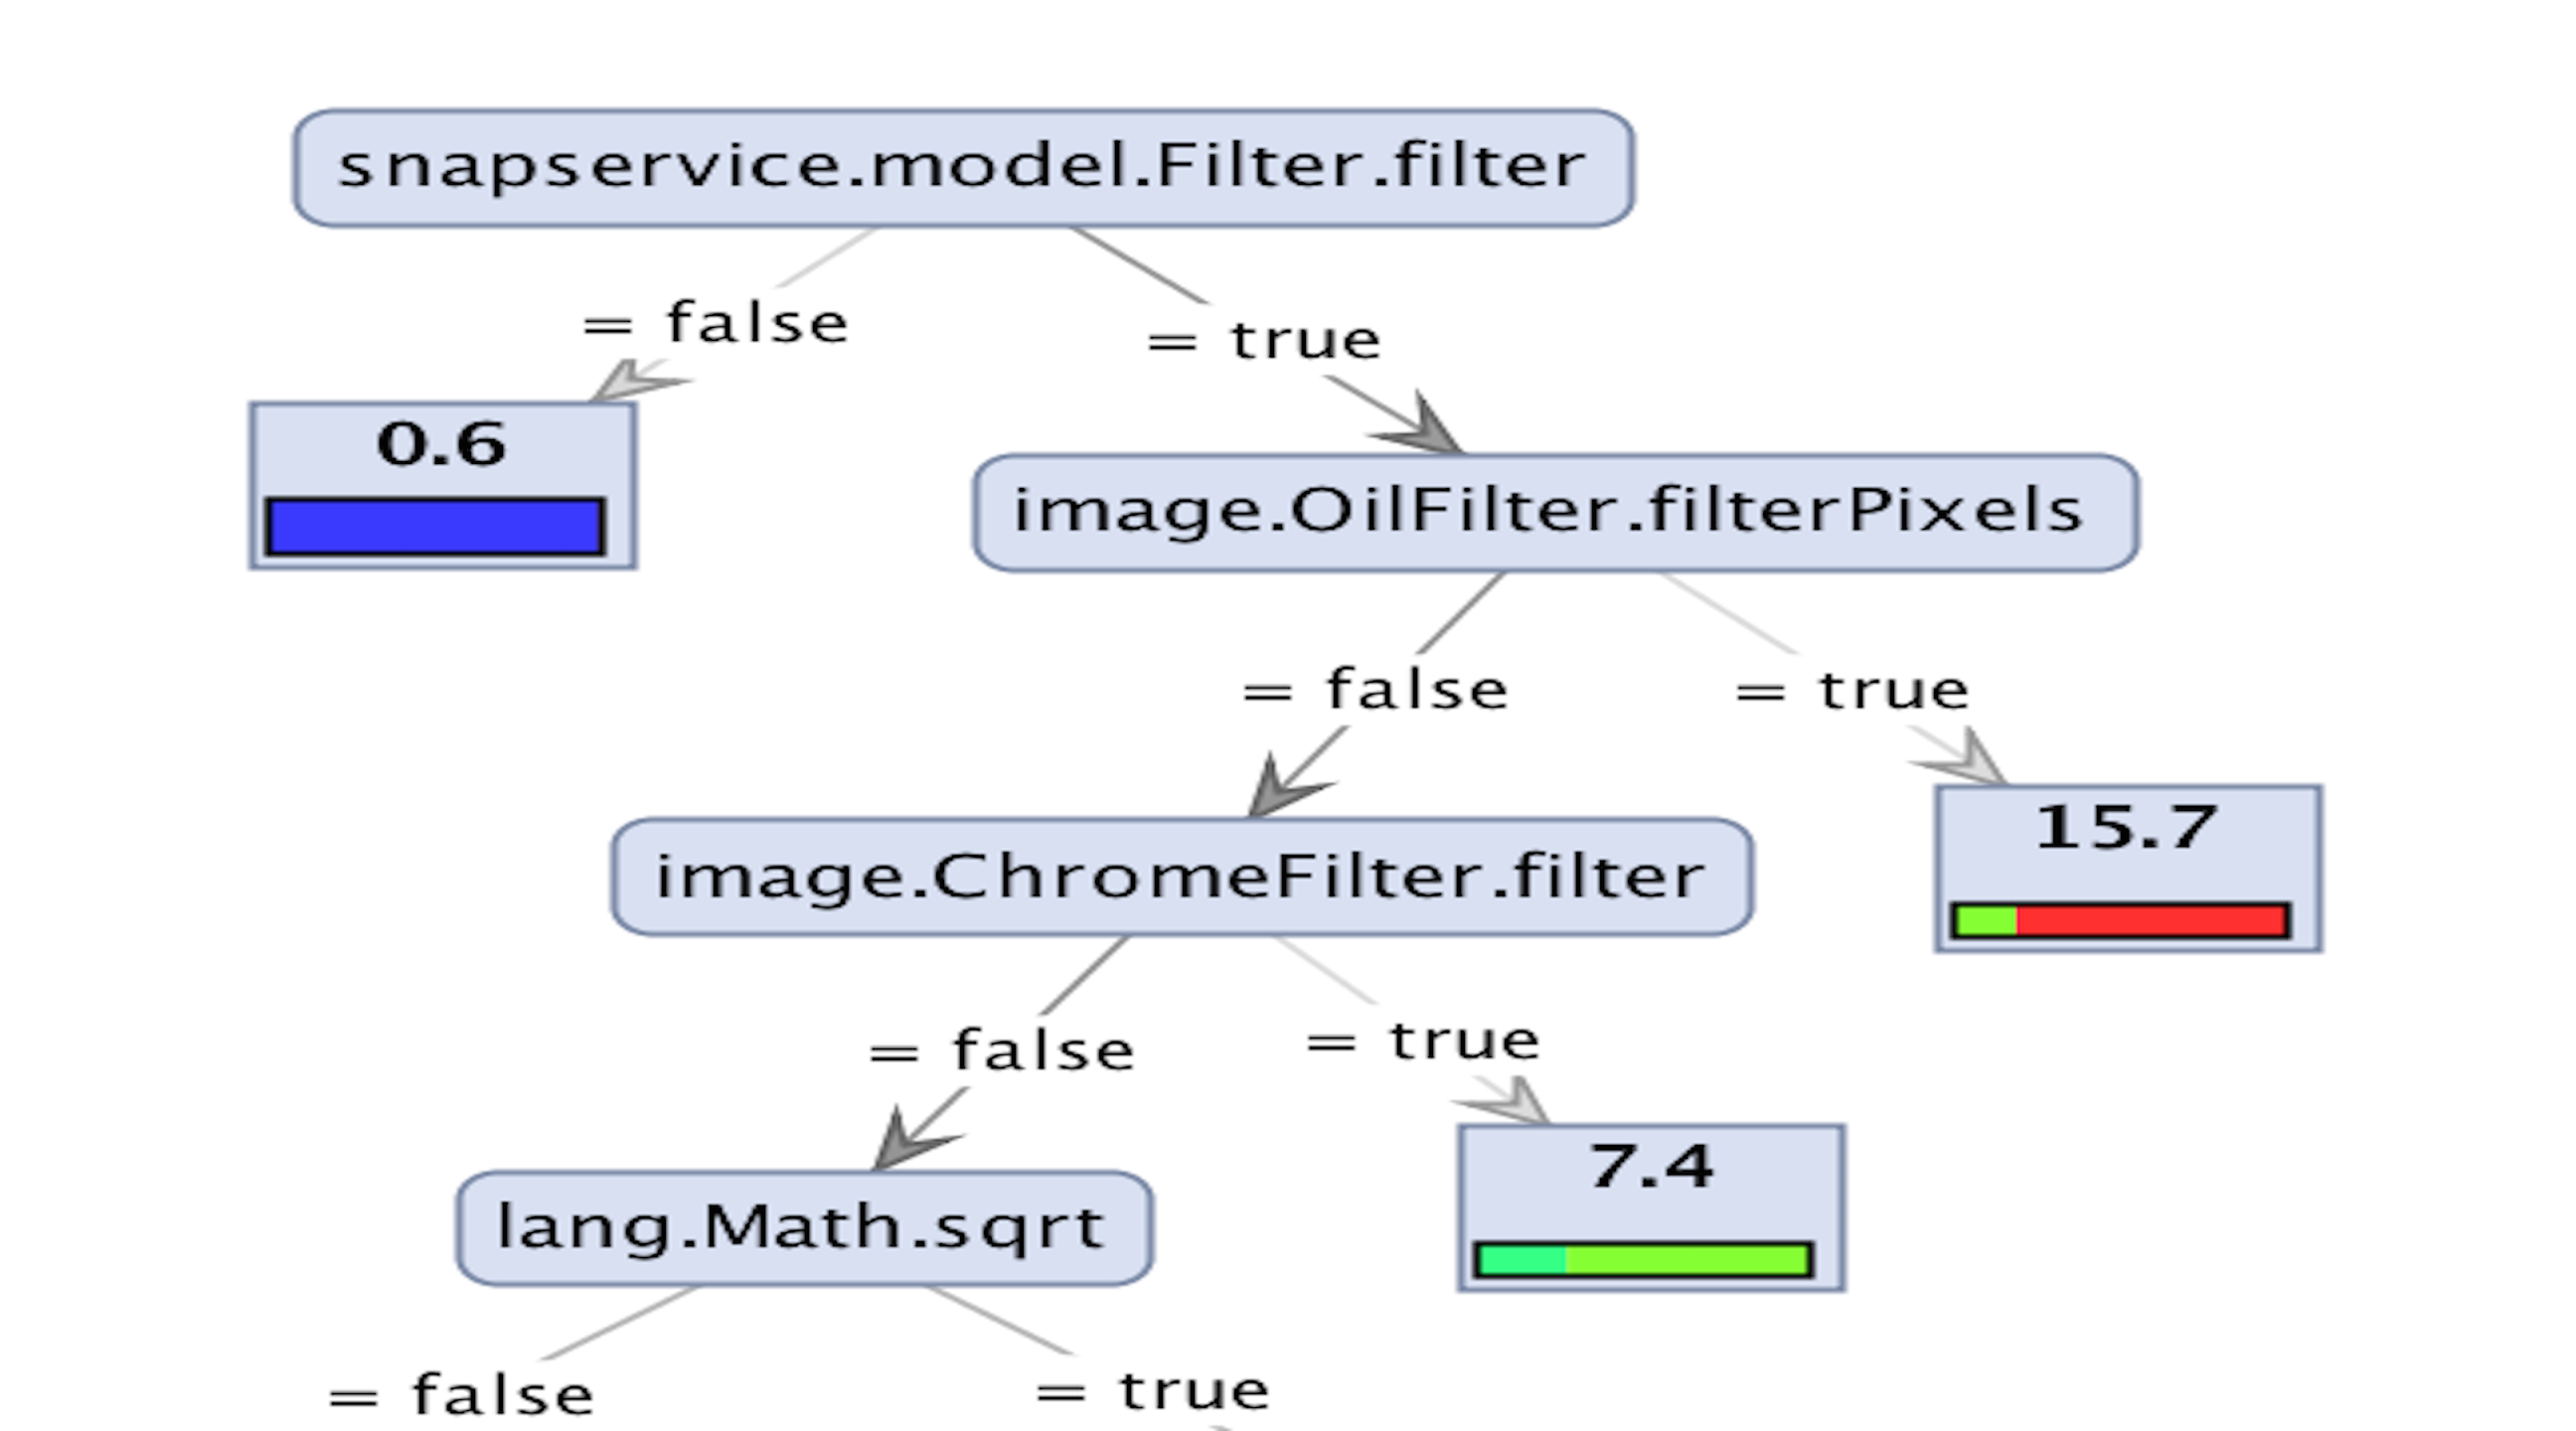
\includegraphics[width=\textwidth]{SnapBuddy_DecisionTree_1}
  \caption{Snippet of a decision-tree discriminant learned from SnapBuddy traces using the timing labels from Figure~\ref{fig:sbtime}.}
  \label{fig:sbdectree}
\end{minipage}
\vspace{-1em}
\end{figure}

Figure~\ref{fig:sbdectree} shows part of discriminant model explains timing differences
based on SnapBuddy functions. 
For instance, the cluster representing the longest running time (around $15$ seconds) is
discriminated by calling functions of \texttt{snapservice.model.Filter.filter} and 
\texttt{image.OilFilter.filterPixels}, indicating that the two methods
are both invoked by the trace. Likewise, the cluster representing the
running time around $7.5$ seconds is discriminated by the
property \texttt{snapservice.model.Filter.filter} and
not \texttt{image.OilFilter.filterPixels} and
\texttt{image.ChromeFilter.filter}, indicating that
\texttt{image.OilFilter.filterPixels} must not invoked
while the other two are.

The analyst might now suspect what is going on: the timing
differences are caused by the filters that each user chooses to apply
to their picture. %To illustrate the filters, Figure~\ref{figure2-1}
%shows a user's image transformed by the Chrome filter (middle) and Oil
%filter (right).
Note that the analyst running the tool did not need to
know that the filters are important for causing this time differential, or even that
they existed. The tool discovers them simply because the trace
contains all method calls. A possible fix now suggests itself:
make sure that the execution of
each type of filter takes the same amount of time.

\section{Methodology}
In this section, we explain the steps and process to produce a discriminant
decision tree model using the example of SnapBuddy described in the previous
section. Figure \ref{Methodology} shows the steps of processing on the SnapBuddy
example. As we described in the previous sections, the records (traces ) of data sets from
input applications include time measurements (uninstrumented version) and function
calls (instrumented version using Soot Framework) under the same user input. As noted before,
we are interested in seeing whether the key
methods that explain the differences in execution time can be pinpointed. Thus, we
consider attributes corresponding to the called methods in a trace. This data set for SnapBuddy
is the input for the process model of Figure \ref{Methodology} (note that the Figure shows
only part of function calls). 
Let's look at the process step by step: \\
1. \smallskip\textit{Clustering and Class Label: Total Execution Time Ranges.}
To identify the most salient attributes, we fix a small number of possible
labels, and cluster traces according to total execution time. 
Each cluster is defined by a corresponding time interval. The clusters and
their intervals are learned using $k$-means clustering
algorithm. In this case, we fix $k$=6 and cluster the data set as shown in the
result of $step.1$. We consider the execution time for each trace to be a
random variable and assume a normal distribution.
We obtain the mean and variance through $10$ repeated measurements.
We apply clustering to the mean execution times of each trace to
determine the class labels. A class label (or cluster) can be identified by the mean of
all execution times belonging to that cluster. Then, considering the
class labels sorted in increasing order, we define the lower boundary
of a bucket for classifying new traces by averaging the maximum
execution time in the previous bucket and the minimum execution time
in this bucket (and analogously for the upper boundary). 
\begin{figure}[t]
    \centering
    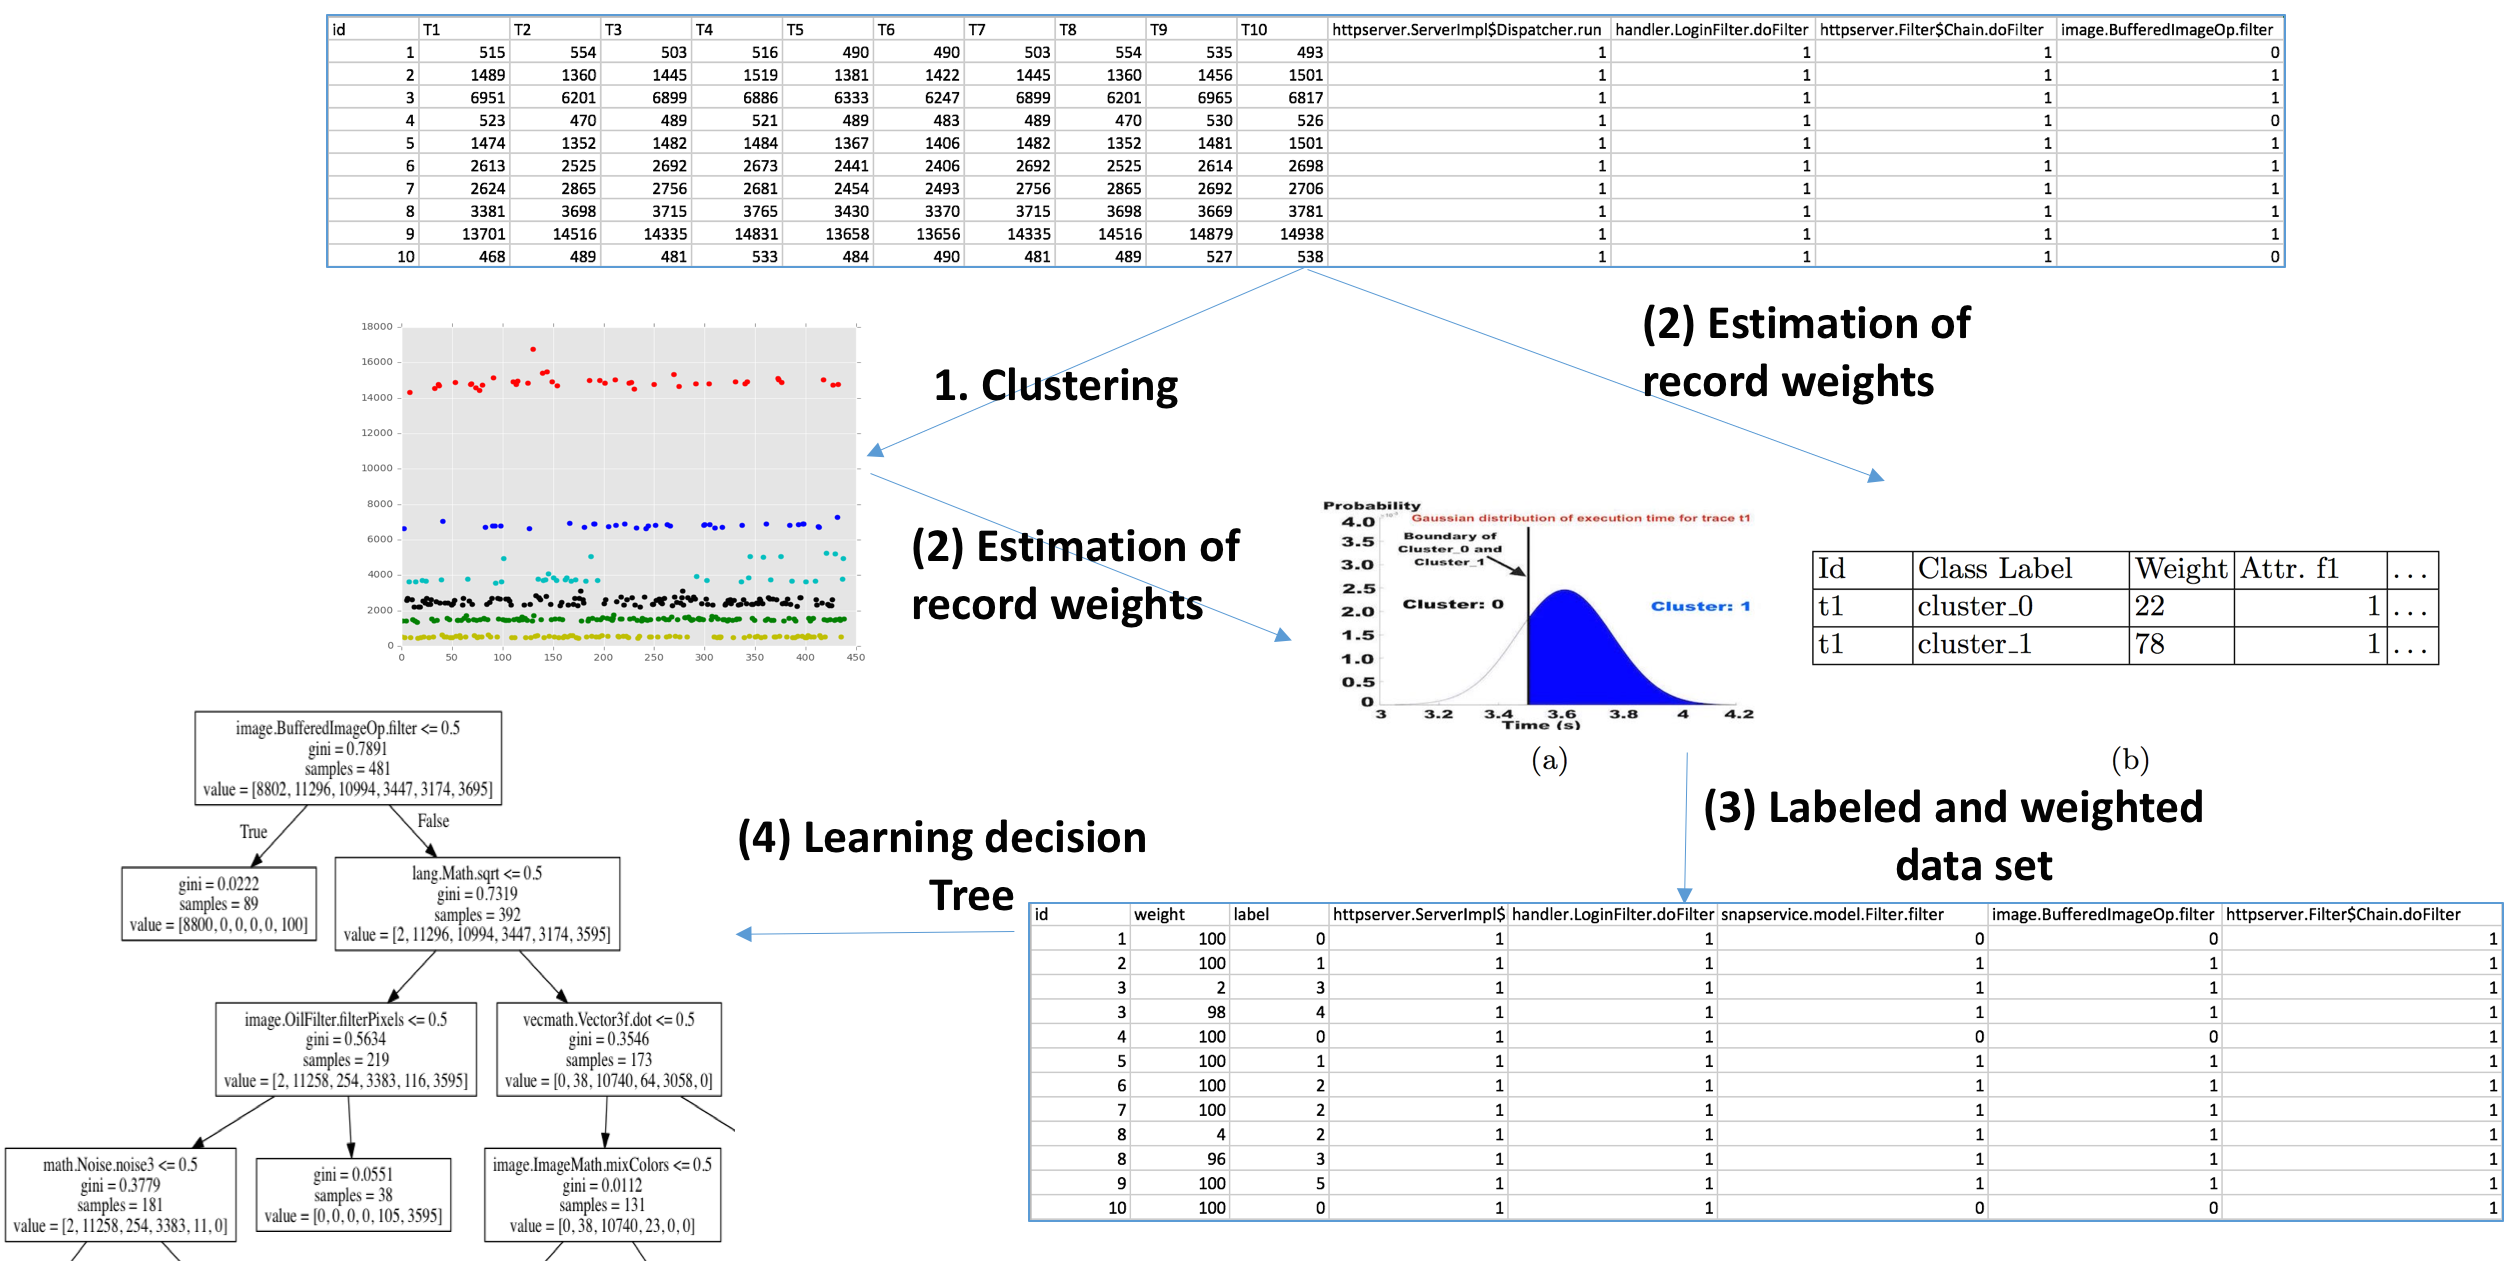
\includegraphics[width=1\textwidth]{Methodology}
    \caption{An overall view of the tool's process for clustering and classification of input data set}
    \label{Methodology}
\end{figure}
\\2. \smallskip\textit{Estimation of trace weights.}
Given a set of time ranges, we define a weighted labeling of traces
that permits a trace to be assigned to different clusters with different weights.
For a given trace, the weights to clusters are determined by the
probability mass belong to the time range of the cluster.  For
example, consider the execution time distribution of a sample trace t1
(drawn from our SnapBuddy example discussed below) shown in
this step. This distribution straddles the
cluster$\_$0 and cluster$\_$1 boundary.  In this case, we assign trace
t1 to both cluster$\_$0 (black area) and cluster$\_$1 (blue area) with
weights according to their probability mass in their respective
regions. In this example, trace t1 is assigned
to cluster$\_$0 with weight 22 and cluster$\_$1 with weight 78. Note
that this provides a smoother interpretation of the class labels
rather than, for example, assigning the most likely label for each
trace. Please note that the tool can also handle the case where
there is just one time measurement, and each trace belongs to a
fix cluster. \\
3. \smallskip\textit{data set of trace labels and weights.}
Given that the first step will assign labels on traces and the second step
calculate the weight of the trace to belong to different labels,
we can obtain the new data set which is the input for classification step. 
We keep the function call features like the original input data set, but we
find labels and weights for each trace as described in the second and third steps
and generate the data set as shown in this step for SnapBuddy. \\
4. \smallskip\textit{Decision Tree Learning.}
From a training set with this weighted labeling, we apply the weighted
decision tree learning algorithm CART. We use group k-fold cross
validation procedure to find accuracy. 
\begin{figure}[t]
    \centering
    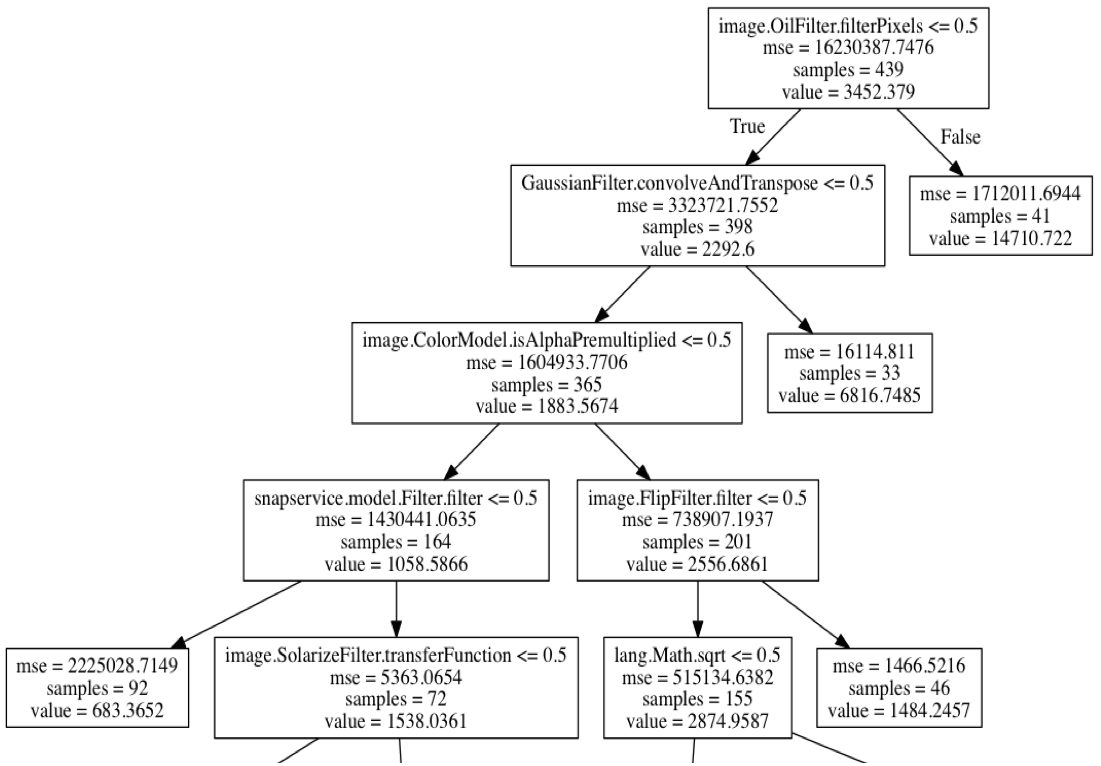
\includegraphics[width=0.8\textwidth]{Regression_Tree}
    \caption{Regression Tree: Results of applying regression tree algorithm on SnapBuddy}
    \label{Regression_Tree}
\end{figure}

The another approach is to apply regression tree directly. Especially,
we know that time is continuous domain. Therefore, we can naturally
apply regression tree on our data sets. Figure \ref{Regression_Tree}
shows the results of applying regression tree on SnapBuddy data set.
As you may notice, on each leaf node, we have the predicted value for
time. For example, if $image.OilFilter.filterPixels$ is called (the right child taken), 
then the predicted time value is about 14.7 seconds which corresponds to
traces which called $oilFilter$ function. In the case of decision tree classifier,
the leaf node classifies the path to one of possible labels. 



\section{Estimation of Cluster Numbers}
In order to apply classifiers with higher accuracy, in some applications, we need to have a rough estimation of how many clusters can be form in the given dataset. Therefore, we choose DBSCAN to estimate the number of clusters. Density-based spatial clustering of applications with noise groups data samples by identifying core points and their reachable neighbors.
The idea behind the algorithm of DBSCAN can be elaborated as the following:
\begin{enumerate}
    \item
    Determining two parameters $\epsilon$ and the minimum number of samples required to form a cluster. In our implementation, we define $\epsilon=0.3$ and the number of minimum samples is 10.
    \item
    The algorithm scan each data sample that hasn't been marked unvisited, find $\epsilon-neighbors$ of this point, if the number of points reach the minimum baseline, a new cluster is formed. Otherwise, this point is marked as noise with label $-1$ in our implementation.
    \item
    If a point in $\epsilon-neighbors$ is also the core point of another cluster, we union these two clusters to form a new one.
    \item
    The above processes repeats until all data samples are visited and therefore, we get the dataset being clustered with different labels.
\end{enumerate}
We apply the DBSCAN algorithm in our micro-benchmark applications. The applications are set of vulnerable programs to side-channels. It takes different time for different function calls, and the function calls are correlated with secret information. The input of the application is a set of bit sequence of 0 and 1. Given the inputs, the programs will call functions which are determined by pattern of the benchmark:
1- \textbf{MSB} which calls only one function given every input. The function call is corresponding to the most significant set bit in the input. As a result, this application leaks the location the most significant 1-bit. This application contains 10 functions.
2- \textbf{Reg} which looks for a given patterns in the input and calls several functions corresponds to the matched pattern in the input. RegEx\_20, RegEx\_150 and RegEx\_200 are applications with 20, 150 and 200 different function calls, looking for patterns 101, 10011 and 101011 respectively. This application will leak whether the pattern occurs in the input and if it is, it will leak the location of the pattern. 
Table \ref{tabel5-1} shows the results of applying DBSCAN algorithm on the micro-benchmark.
The result shows that the number of clusters may not be equal to number of function in the benchmarks
even if each function has different and unique execution time.
\begin{table}[t]
  \centering
    \caption{Estimation of cluster numbers using DBSCAN
   }
  \label{tabel5-1}
\begin{tabular}
{ |p{3.5cm}||p{1.6cm}|p{1.6cm}|p{1.6cm}|p{1.6cm}| }
 \hline
 \multicolumn{5}{|c|}{DBSCAN Results} \\
 \hline
 Measurements & MSB1\_10 & RegEx\_20 &RegEx\_150 & RegEx\_200\\
 \hline
 Est. Num. Clusters   & 9 & 6 & 51 & 69\\
 Homogeneity & 0.499 & 0.333 &0.496 & 0.489\\
 Completeness & 1.000 & 1.000 & 1.000 & 1.000\\
 V-measure & 0.666 & 0.500 & 0.663 & 0.656\\
 Adjusted Rand Index & 0.187 & 0.003 & 0.001 & 0.000\\
 Silhouette Coefficient & 1.000 & 0.616 & 0.791 & 0.718\\
 \hline
\end{tabular}\\
\end{table}
Considering the measurements of Table \ref{tabel5-1}, the following explains the measurements: 
\textit{Homogeneity} explains the purity of data in clusters. Therefore, the higher homogeneity score is the better performance of clustering algorithm has. \textit{Completeness} explains whether a cluster contains all the data points of a given class. \textit{V-measure} is the harmonic mean between homogeneity and completeness. A perfect labeling is 1.0. \textit{Rand Index} is very low here since the input matrix is sparse. Therefore, it thinks samples in the same class are classified into different classes.
\textit{Silhouette} Coefficient is the highest for cluster numbers where the inter-cluster distances are the biggest and intra-cluster distance is the smallest.  

\section{Other Regression and Classifiers}

\begin{enumerate}
    \item Regression.
    For linear regression, we split 80\% of each data into training set. By fitting the data in a regression model we get the following scores. The accuracy of MSB data is almost 1.0 since linear pattern is very obvious with only one function call at each time. But for other data sets, the linear
    regression could not explain data with high accuracy. Table \ref{tabel6-1} shows the performance of
    linear regression on micro-benchmark applications. 
    \item Classification.
    For classification problems we applied nearest neighbors, linear SVM, RBF SVM, random forest, neural network, ada-boosting and Naive bayes classifiers. Table \ref{tabel6-2} indicates that naive bayes, nearest neighbors and RBF SVM have the best performance.
\end{enumerate}
\begin{table}[t]
  \centering
    \caption{Linear Regression model performance on micro-benchmark applications}
  \label{tabel6-1}
\begin{tabular}{ |p{3cm}||p{1.8cm}|p{1.8cm}|p{1.8cm}|p{1.8cm}| }
 \hline
 \multicolumn{5}{|c|}{Linear Regression Model} \\
 \hline
 Scores & MSB1\_10 & RegEx\_20 &RegEx\_150 & RegEx\_200\\
 \hline
 Variance Score   & 0.99 & 0.97 & -1.63e+19 & -2.22e+19\\
 MSE & 2.28 & 4870613.93 & $2.26*10^{29}$ & $1.16*10^{30}$\\
 \hline
\end{tabular}\\
\end{table}

\begin{table}[t]
  \centering
    \caption{Performance of different classifiers on micro-benchmark applications}
  \label{tabel6-2}
\begin{tabular}{ |p{3cm}||p{1.8cm}|p{1.8cm}|p{1.8cm}|p{1.8cm}| }
 \hline
 \multicolumn{5}{|c|}{Linear Regression Model} \\
 \hline
 Scores & MSB1\_10 & RegEx\_20 &RegEx\_150 & RegEx\_200\\
 \hline
 Nearest Neighbors   & 1.0 & 0.1 & 0.08 & 0.09\\
 Linear SVM & 0.56 & 0.1 & 0.03 & 0.06\\
 RBF SVM & 1.0 & 0.2 & 0.1 & 0.11\\
 Random Forest & 0.98 & 0.17 & 0.08 & 0.06\\
 Neural Net & 0.98 & 0.2 & 0.04 & 0.07\\
 Adaboost & 0.98 & 0.2 & 0.03 & 0.06\\
 Naive Bayes & 1.0 & 0.23 & 0.09 & 0.09\\
 \hline
\end{tabular}\\
\end{table}


\section{Results}
As described earlier, we are looking for a scalable and accurate model which should
be able to explain the data given program internal function calls as features and time
of trace execution as the target. We observe that decision tree classifier and
regression tree give a reasonable explanation for the input data and have good
accuracy and high scalability. We also consider the compactness of model in
terms of height of tee. Table \ref{table7-1} shows the results of applying decision
tree classifier on the applications and micro-benchmarks we have used in this project.
It is worth nothing to mention that explaining the data with good accuracy is more
important to us in comparison to less explanatory models with high accuracy.

\begin{table}[t]
  \centering
  \caption{Application and Micro-benchmark results for decision-tree discriminators. 
    Legend: \textbf{\#M}: number of methods, \textbf{\#N:} number of traces,
    \textbf{T}:\ computation time in seconds, \textbf{A}: accuracy, 
    \textbf{H}: decision-tree height % denotes a time less than
    %$0.1$ seconds.
   }
  \label{table7-1}
  \begin{tabular}{ || l | r | r || r | r | r ||}
    \hline
    &       &    & \multicolumn{3}{c||}{Decision Tree}\\
    ~~~~Application Name~~~~~~ & \# \textbf{M} & \#\textbf{N} & \textbf{T} & \textbf{A} & \textbf{H} \\ \hline
     $Existing User Enumeration$ & 2 & 1000 & 0.01 & 100\% & 2  \\ \hline
    $SnapBuddy$ & 160 & 439 & 0.01 & 100\% & 8  \\ \hline
    $MSB0$ & 10 & 188 & 0.01 & 100\% & 7  \\ \hline
    $RegE_{101}$ & 20 & 200 & 0.01 & 100\% & 13 \\ \hline
    $RegE_{10011}$ & 150 & 1500 & 0.5 & 89.2\% & 44  \\ \hline
    $RegE_{101011}$ & 200 & 2000 & 0.8 & 92.1\% & 50 \\ \hline
    \end{tabular}
\end{table}

\section{Conclusion}
In this project, we show that combination of program analysis and machine learning can help
security analysts to find explanation for possible execution time difference in program
control flow paths. We show our approaches with two real applications and micro-benchmarks.
In particular, we show that clustering data in time domain (obtaining class labels) and classification
of them using decision tree discriminant is a useful approach to explain time difference.
We also show that regression tree ca be also useful to explain the timing differences. 
One challenge includes finding the number of clusters in the data set. We use DBSCAN to
estimate cluster numbers. We also provide the performance of other machine learning algorithm but they are less explainable. Possible extensions include considering the case such
that order of function calls is important. The another extension is to compare two approaches: (1) clustering and then classification, (2): direction regression models.

\end{document}
